%%____________________________________________________________________________||
\section{Signal injection test}
\label{sec:sig-injection}
In this appendix we report the results of the signal injection test. The procedure used is described in the following.

For each inspected signal strength $\mu=\sigma_{sig,inj}/\sigma_{sig,theory}$ 3000 thousand toys are generated using post-fit nuisances (``frequentist toys'').
For each toy the signal strength is fitted while all the other nuisance parameters are profiled, 
with the same procedure used to compute upper limits presented in Sec.~\ref{sec:susy}, \ref{sec:darkmatter}.
For each value of the injected signal the median of the distribution of best fit values from toys is extracted and plotted against the injected value. 
A linear fit including all the points is performed in order to check if the likelihood gives a linear un-biased response. 
For this linear fit, only the statistical uncertainty on the median is used. \\
The results are presented in Fig.~\ref{fig:sigInj} for two Dark Matter models. 
The parameters of the linear fit are compatible with a linear response. 

\begin{figure}[h!] 
  \centering
  \subfigure[Axial-vector $m_{\phi}=1500$ GeV, $m_{DM}=50$ GeV]{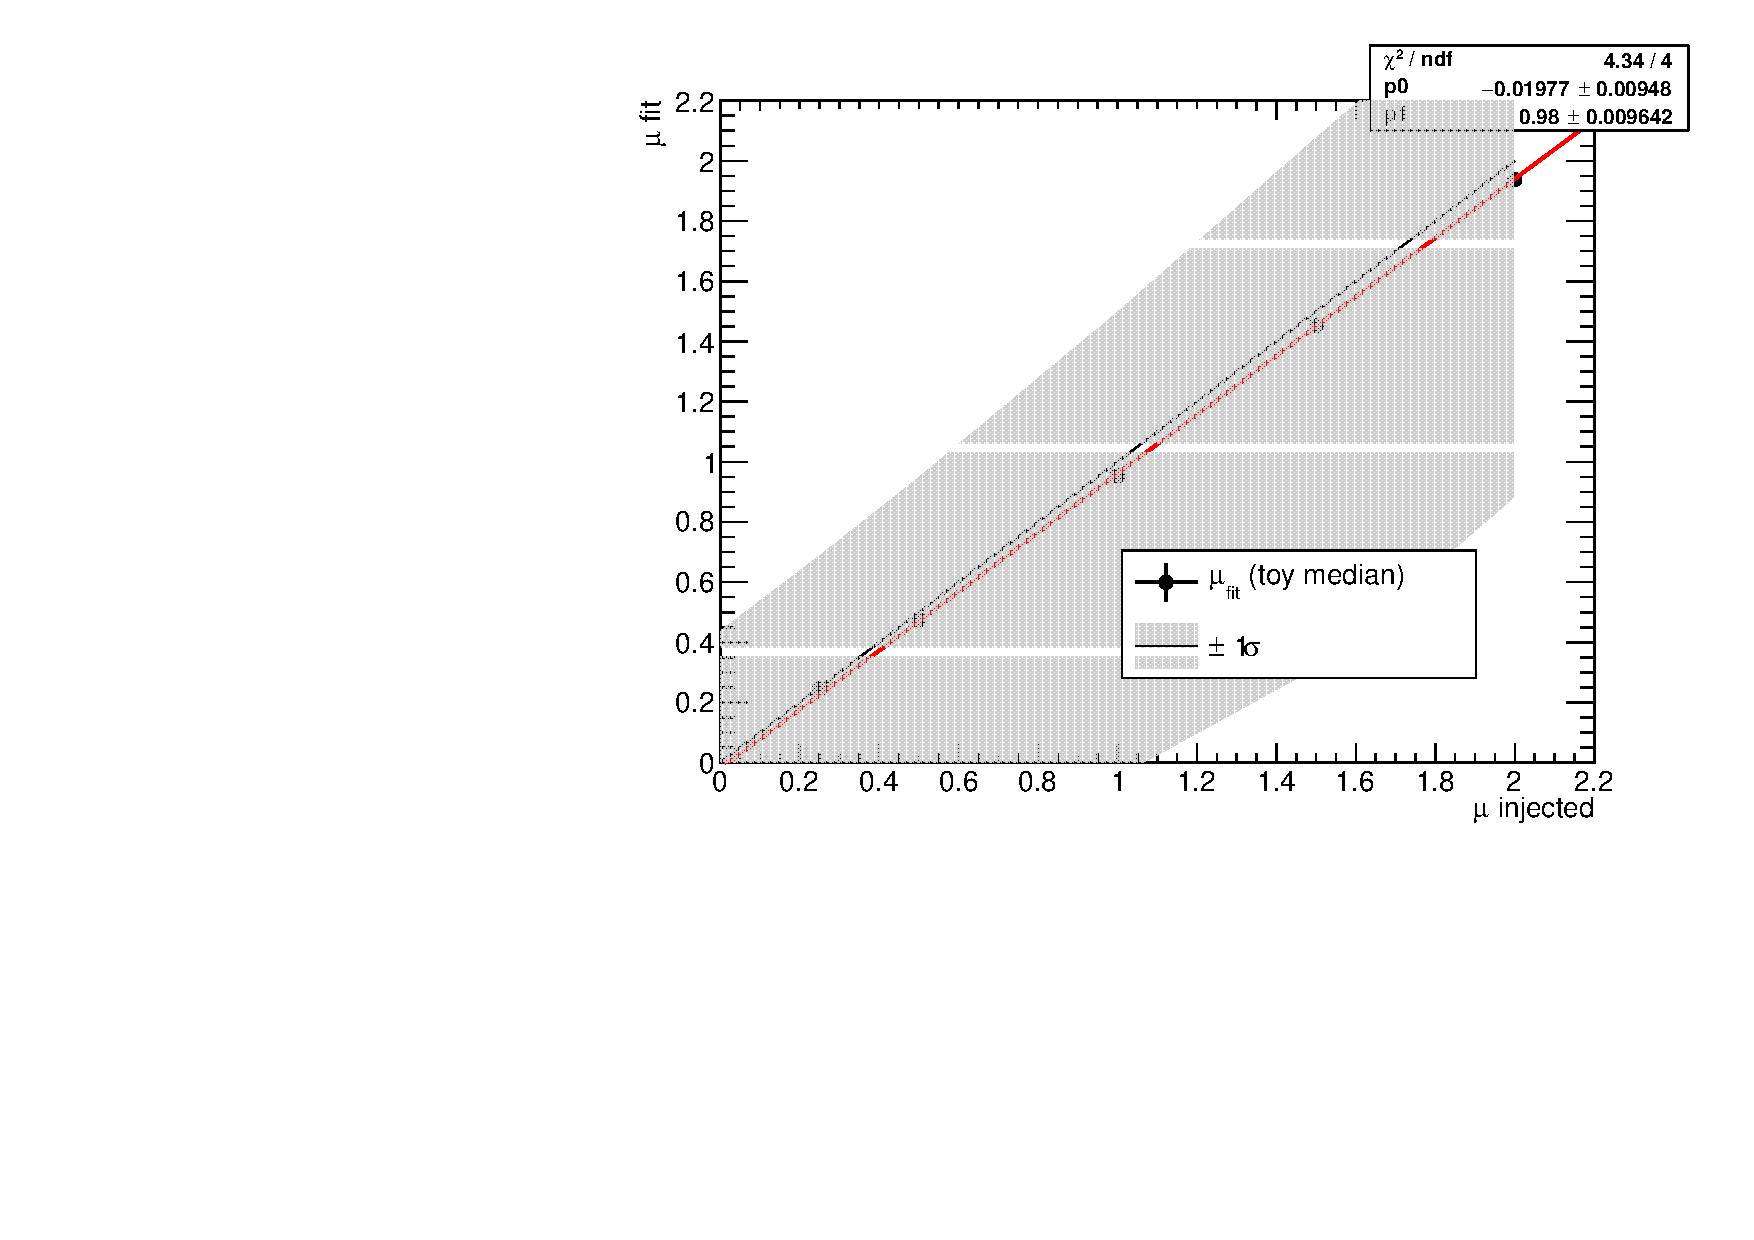
\includegraphics[width=0.45\textwidth]{figures/signalInjection/signalInjection_AV_1500_50}}
  \subfigure[Pseudo-scalar $m_{\phi}=300$ GeV, $m_{DM}=1$ GeV]{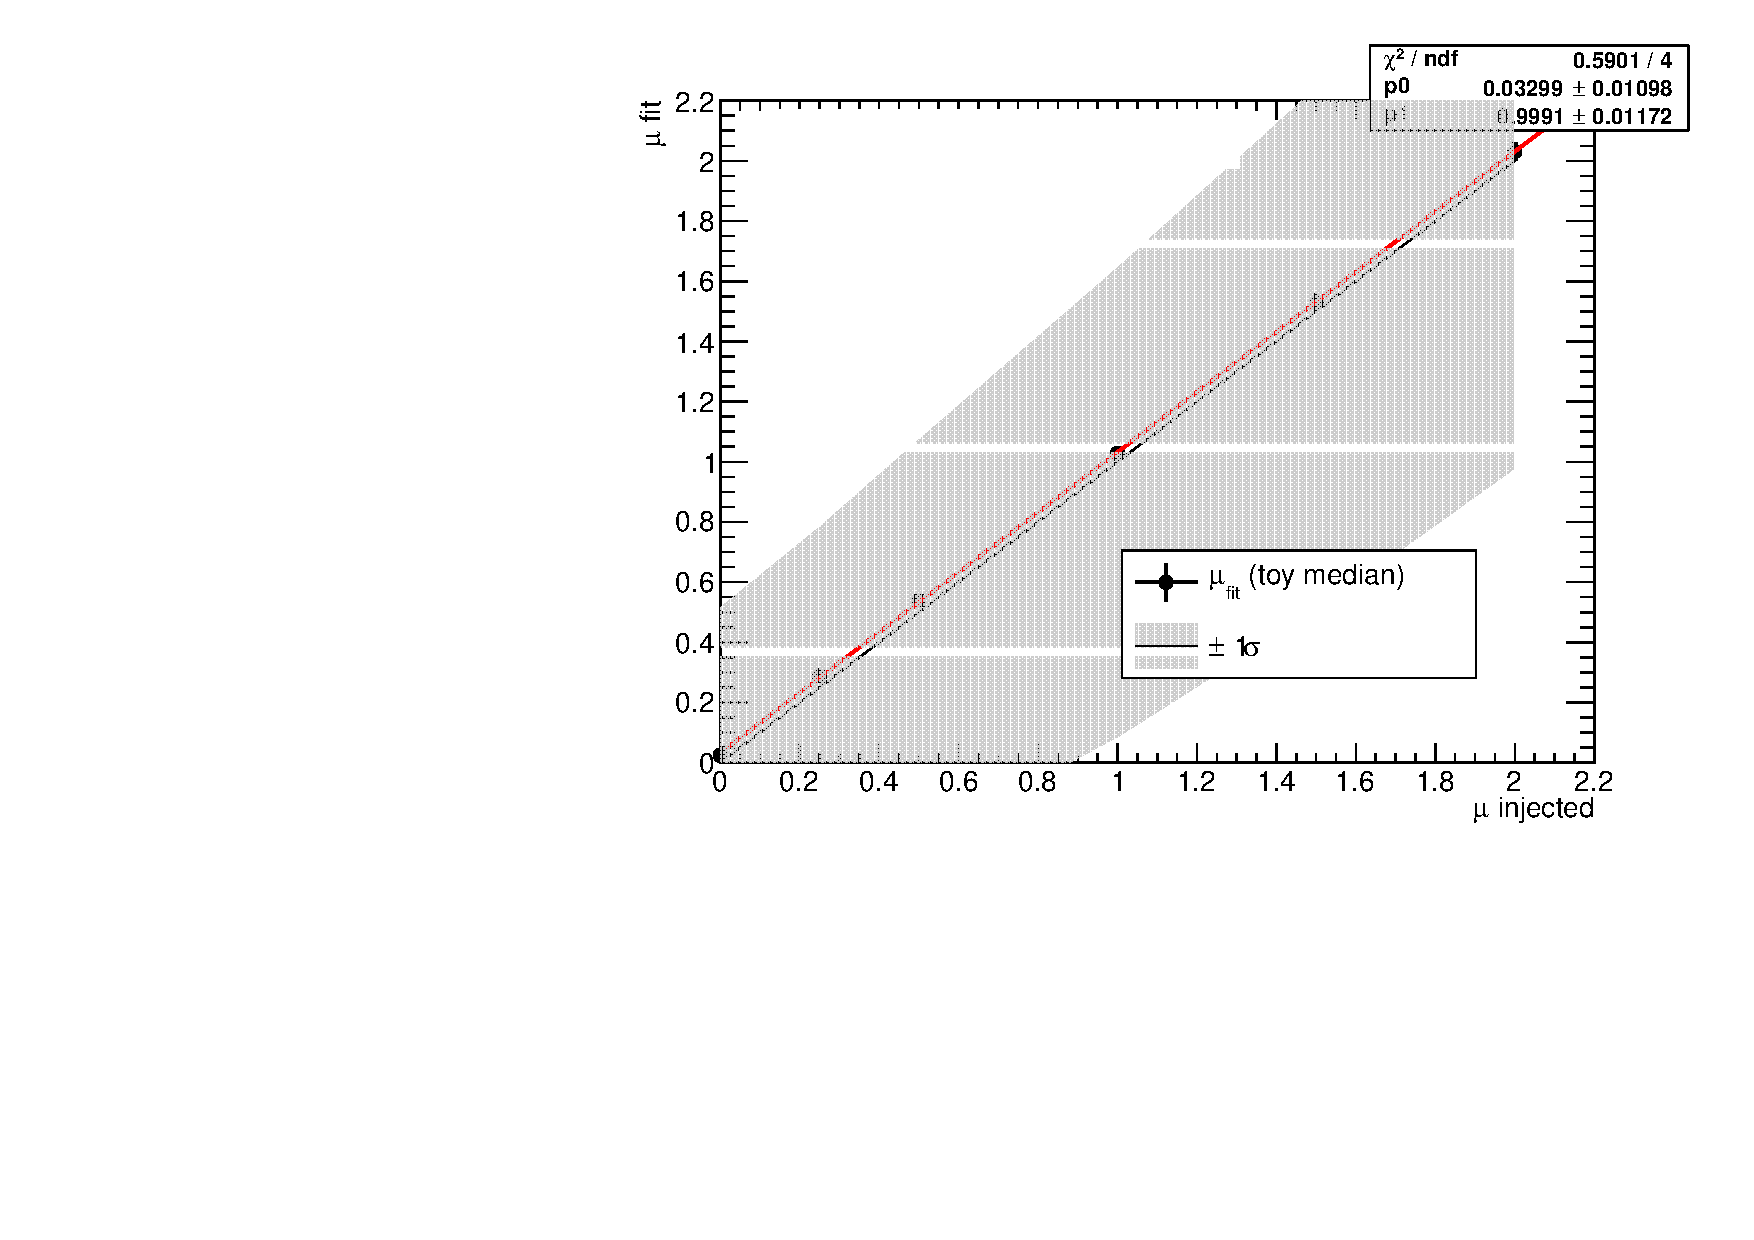
\includegraphics[width=0.45\textwidth]{figures/signalInjection/signalInjection_PS_300_1}}
  \caption{The results of the signal injection test for two Dark Matter models. The black points are the median of the toy distributions corresponding to a given injected signal. 
    The errors represent the statistical uncertainties on the median. The red line shows the result of the linear fit. 
    The grey band respresent the 68\% C.L. interval for the $\mu$ parameter, derived from the quantiles of the toy distribution.}
  \label{fig:sigInj}}
\end{figure}


